\documentclass[tikz,border=10pt]{standalone}
\usepackage[T1]{fontenc}
\usepackage{tgheros}
\usepackage{sfmath}
\usepackage{amsmath}
\usepackage{tikz}
\usetikzlibrary{arrows.meta,positioning,shapes.geometric,fit,backgrounds,calc,patterns}
\usepackage{xcolor}

\renewcommand{\familydefault}{\sfdefault}

% Academic Semantic Palette (Harvard Crimson & ETH Zurich)
\definecolor{ethdarkblue}{HTML}{1F407A}
\definecolor{ethblue}{HTML}{215CAF}
\definecolor{ethbronze}{HTML}{B87333}
\definecolor{harvardcrimson}{HTML}{A51C30}
\definecolor{ethslate}{HTML}{334155}
\definecolor{gridgray}{HTML}{E2E8F0}
\definecolor{safegreen}{HTML}{0D9488}
\definecolor{dangerred}{HTML}{DC2626}

\begin{document}
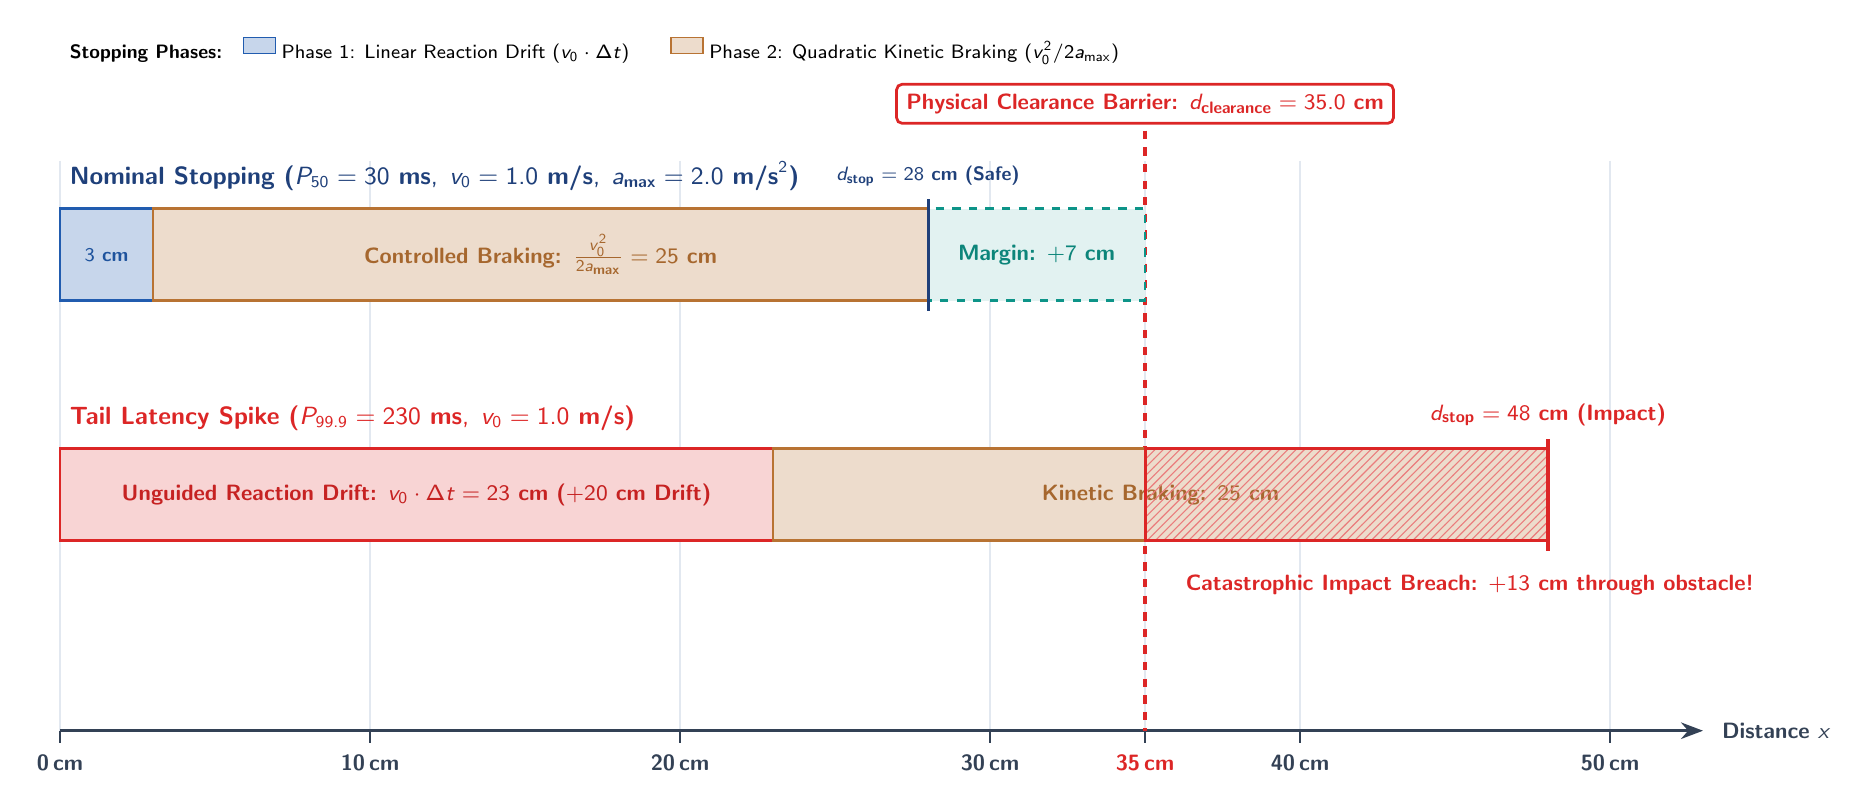
\begin{tikzpicture}[
  font=\sffamily,
  >=Stealth,
  scale=1.0
]

  % ---------------------------------------------------------------------------
  % PARAMETERS: Distance Scale 1 cm = 0.155 in (50 cm = 7.75 in)
  % ---------------------------------------------------------------------------
  \def\xscale{0.155in}
  \def\yNom{0.0in}
  \def\yTail{-1.20in}
  \def\yAxis{-2.15in}
  \def\barH{0.46in}

  % ---------------------------------------------------------------------------
  % BACKGROUND GRID & SPATIAL AXIS
  % ---------------------------------------------------------------------------
  \foreach \x in {0, 10, 20, 30, 40, 50} {
    \draw[gridgray, line width=0.5pt] (\x*\xscale, 0.70in) -- (\x*\xscale, \yAxis);
    \draw[ethslate, line width=0.8pt] (\x*\xscale, \yAxis) -- (\x*\xscale, \yAxis - 0.06in);
    \node[font=\fontsize{8pt}{10pt}\selectfont\bfseries, text=ethslate, below=1pt] at (\x*\xscale, \yAxis - 0.06in) {\x\,cm};
  }

  % 35 cm grid line
  \draw[gridgray, line width=0.5pt] (35*\xscale, 0.70in) -- (35*\xscale, \yAxis);
  \draw[ethslate, line width=0.8pt] (35*\xscale, \yAxis) -- (35*\xscale, \yAxis - 0.06in);
  \node[font=\fontsize{8pt}{10pt}\selectfont\bfseries, text=dangerred, below=1pt] at (35*\xscale, \yAxis - 0.06in) {35\,cm};

  % Spatial Axis Line
  \draw[->, ethslate, line width=1.1pt] (0, \yAxis) -- (53*\xscale, \yAxis)
    node[right=3pt, font=\fontsize{8.5pt}{11pt}\selectfont\bfseries, text=ethslate] {Distance $x$};

  % ---------------------------------------------------------------------------
  % PHYSICAL CLEARANCE BARRIER (x = 35 cm)
  % ---------------------------------------------------------------------------
  \draw[dangerred, dashed, line width=1.5pt] (35*\xscale, 0.85in) -- (35*\xscale, \yAxis);
  \node[draw=dangerred, fill=white, line width=1pt, rounded corners=2pt, inner sep=3.5pt, font=\fontsize{8pt}{10pt}\selectfont\bfseries, text=dangerred, anchor=south] at (35*\xscale, 0.88in) {
    Physical Clearance Barrier: $d_{\text{clearance}} = 35.0\text{ cm}$
  };

  % ---------------------------------------------------------------------------
  % TRACK 1: NOMINAL CASE (P50 = 30 ms -> d_stop = 28 cm)
  % ---------------------------------------------------------------------------
  \node[anchor=south west, font=\fontsize{9pt}{11.5pt}\selectfont\bfseries, text=ethdarkblue] at (0, 0.50in) {
    Nominal Stopping ($P_{50} = 30\text{ ms},\; v_0 = 1.0\text{ m/s},\; a_{\text{max}} = 2.0\text{ m/s}^2$)
  };

  % Phase 1: Reaction Drift (3 cm)
  \draw[fill=ethblue!25, draw=ethblue, line width=0.9pt] (0, \yNom) rectangle ++(3*\xscale, \barH)
    node[midway, font=\fontsize{7.5pt}{9pt}\selectfont\bfseries, text=ethblue!90!black] {$3\text{ cm}$};

  % Phase 2: Kinetic Braking (25 cm: 3 -> 28)
  \draw[fill=ethbronze!25, draw=ethbronze, line width=0.9pt] (3*\xscale, \yNom) rectangle ++(25*\xscale, \barH)
    node[midway, font=\fontsize{8pt}{10pt}\selectfont\bfseries, text=ethbronze!90!black] {Controlled Braking: $\frac{v_0^2}{2a_{\text{max}}} = 25\text{ cm}$};

  % Safe Clearance Margin (7 cm: 28 -> 35)
  \draw[fill=safegreen!12, draw=safegreen, dashed, line width=1.0pt] (28*\xscale, \yNom) rectangle ++(7*\xscale, \barH)
    node[midway, font=\fontsize{8pt}{10pt}\selectfont\bfseries, text=safegreen!90!black] {
      Margin: $+7\text{ cm}$
    };

  % Nominal End Marker
  \draw[ethdarkblue, line width=1.1pt] (28*\xscale, \yNom - 0.05in) -- (28*\xscale, \yNom + \barH + 0.05in);
  \node[font=\fontsize{7.5pt}{9.5pt}\selectfont\bfseries, text=ethdarkblue, above=1pt] at (28*\xscale, \yNom + \barH + 0.05in) {
    $d_{\text{stop}} = 28\text{ cm}$ (Safe)
  };

  % ---------------------------------------------------------------------------
  % TRACK 2: TAIL LATENCY SPIKE (P99.9 = 230 ms -> d_stop = 48 cm)
  % ---------------------------------------------------------------------------
  \node[anchor=south west, font=\fontsize{9pt}{11.5pt}\selectfont\bfseries, text=dangerred] at (0, \yTail + 0.50in) {
    Tail Latency Spike ($P_{99.9} = 230\text{ ms},\; v_0 = 1.0\text{ m/s}$)
  };

  % Phase 1: Expanded Reaction Drift (23 cm)
  \draw[fill=dangerred!20, draw=dangerred, line width=0.9pt] (0, \yTail) rectangle ++(23*\xscale, \barH)
    node[midway, font=\fontsize{8pt}{10pt}\selectfont\bfseries, text=dangerred!90!black] {Unguided Reaction Drift: $v_0 \cdot \Delta t = 23\text{ cm}$ ($+20\text{ cm}$ Drift)};

  % Phase 2: Kinetic Braking (25 cm: 23 -> 48)
  \draw[fill=ethbronze!25, draw=ethbronze, line width=0.9pt] (23*\xscale, \yTail) rectangle ++(25*\xscale, \barH)
    node[midway, font=\fontsize{8pt}{10pt}\selectfont\bfseries, text=ethbronze!90!black] {Kinetic Braking: $25\text{ cm}$};

  % Barrier Breach Hatch (35 -> 48 cm)
  \draw[pattern=north east lines, pattern color=dangerred!60, draw=dangerred, line width=1.1pt] 
    (35*\xscale, \yTail) rectangle (48*\xscale, \yTail + \barH);

  % Breach Callout Text
  \node[font=\fontsize{8.5pt}{10.5pt}\selectfont\bfseries, text=dangerred, anchor=west] at (36*\xscale, \yTail - 0.22in) {
    Catastrophic Impact Breach: $+13\text{ cm}$ through obstacle!
  };

  % Tail End Marker
  \draw[dangerred, line width=1.2pt] (48*\xscale, \yTail - 0.05in) -- (48*\xscale, \yTail + \barH + 0.05in);
  \node[font=\fontsize{8pt}{10pt}\selectfont\bfseries, text=dangerred, above=1pt] at (48*\xscale, \yTail + \barH + 0.05in) {
    $d_{\text{stop}} = 48\text{ cm}$ (Impact)
  };

  % ---------------------------------------------------------------------------
  % LEGEND (Top row of clean semantic pills)
  % ---------------------------------------------------------------------------
  \coordinate (L0) at (0, 1.25in);
  \node[anchor=west, font=\fontsize{7.5pt}{9.5pt}\selectfont] at (L0) {
    \textbf{Stopping Phases:}\quad
    \tikz[baseline=-2pt]{\draw[fill=ethblue!25, draw=ethblue] (0,0) rectangle (0.16in, 0.08in);}\;Phase 1: Linear Reaction Drift ($v_0 \cdot \Delta t$)\qquad
    \tikz[baseline=-2pt]{\draw[fill=ethbronze!25, draw=ethbronze] (0,0) rectangle (0.16in, 0.08in);}\;Phase 2: Quadratic Kinetic Braking ($v_0^2 / 2a_{\text{max}}$)
  };

\end{tikzpicture}
\end{document}
